\documentclass{beamer}
\usepackage[utf8]{inputenc}

\usetheme{Madrid}
% \usecolortheme{seahorse}

% For Polish langage
\usepackage[T1]{fontenc}
% \usepackage[polish]{babel}
\usepackage{tikzsymbols}

% For strikethrough text
\usepackage{ulem}

% For tables
\usepackage{multirow}
\usepackage{pdflscape}
\usepackage{colortbl}
\usepackage{tabulary}
\usepackage{etoolbox}
\usepackage{makecell}
\newcolumntype{P}[1]{>{\centering\arraybackslash}p{#1}}

% For figures
\usepackage{caption}
\usepackage{subcaption}

% For math
\usepackage{amsmath,amsfonts}

% For inline code listings
\usepackage{listings}
\usepackage{xparse}
\usepackage{xcolor}
\lstdefinestyle{py}{
  language=Python,
  basicstyle=\small\ttfamily,
  commentstyle=\color{green!40!black},
  keywordstyle=\color{blue},
  numberstyle=\tiny\color{gray},
  numbers=left,
  numbersep=5pt,
  backgroundcolor=\color{white},
  showspaces=false,
  showstringspaces=false,
  frame=single,
  rulecolor=\color{black},
  tabsize=4,
  captionpos=b,
  breaklines=true,
  breakatwhitespace=true,
  title=\lstname,
  caption=\lstname
}

% For algorithms
\usepackage{algorithm,algpseudocode}

\usepackage[backend=biber]{biblatex}
\addbibresource{references.bib}

% Arrows
\usepackage{tikz}
\usetikzlibrary{shapes.arrows}
\tikzset{
    myarrow/.style={
        draw,
        fill=orange,
        single arrow,
        minimum height=5ex,
        single arrow head extend=1ex
    }
}
\newcommand{\arrowup}{\tikz [baseline=-0.5ex]{\node [myarrow,rotate=90] {};}}
\newcommand{\arrowdown}{\tikz [baseline=-1ex]{\node [myarrow,rotate=-90] {};}}

% Title page
\title[IC2S2 2024]{10th International Conference on Computational Social Science}
\subtitle{Network Diffusion --- Framework to Simulate Spreading Processes in Complex Networks}
\author[Micha{\l} Czuba et al.]{
    \textbf{Micha{\l} Czuba} \inst{1},
    Mateusz Nurek \inst{1},
    Damian Serwata \inst{1},
    Yu-Xuan Qi \inst{2},
    Mingshan Jia \inst{2},
    Katarzyna Musial \inst{2},
    Rados{\l}aw Michalski \inst{1},
    Piotr Br{\'o}dka \inst{1}
}
\institute[]{
  \inst{1} Wroc{\l}aw University of Science and Technology\\
  \inst{2} University of Technology Sydney
}
\date[20.07.2024]{20.07.2024}
\logo{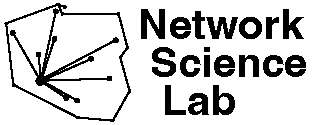
\includegraphics[height=0.5cm]{figures/nsl.pdf}}

\AtEndDocument{
    \addtocounter{framenumber}{-1}
    \begin{frame}[c]
        \centering
        \begin{huge}
            Thank you for your attention!
        \end{huge}
        \begin{figure}
            
\includegraphics[width=5cm]{figures/qr_code2.pdf}
        \end{figure}
        Scan this QR code to reach the main page of the project \Smiley
    \end{frame}
}

\begin{document}

\frame{\titlepage}

\begin{frame}{Agenda}
    \tableofcontents
\end{frame}

\section{Motivation}

\begin{frame}{\secname}
    Spreading phenomena are one of the problems considered by a network science. They can be obeserved
    in various areas like: dynamics of political opinions, marketing campaigns, spread of epidemics,
    computer viruses, etc.
    \begin{figure}
        \centering
        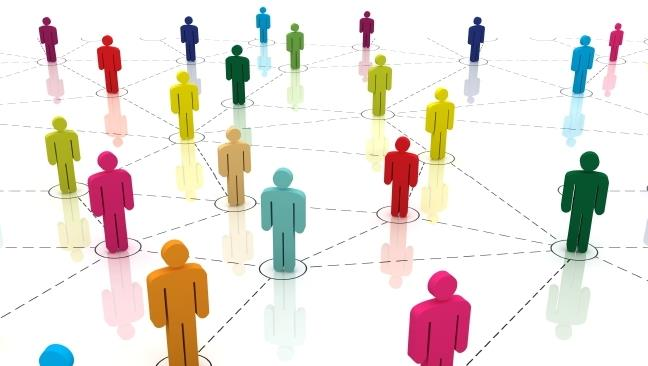
\includegraphics[width=.7\textwidth]{figures/social_network.jpg}
        \caption{Artistic representation of a social network.\footnote{Source: \url{
        www.uniroma3.it/articoli/seminario-biased-opinion-dynamics-when-the-devil-is-in-the-details-138122}
        }}
    \end{figure}
\end{frame}

\begin{frame}{\secname}
    \onslide<1->{Analytical approaches to such phenomena are often insufficient for large graphs,
    prompting researchers to use computational methods, i.e. simulations.}
    \onslide<2->{\begin{center}
        \vspace{1em}
        \arrowdown
        \vspace{1em}
    \end{center}
    Thus, many tools were developed to address that issue, allow researchers to get rid of the need
    to start their experiments from scratch, and enhance the reproducibility of results.}
\end{frame}

\begin{frame}{\secname}
    \begin{columns}[T]
        \begin{column}{.35\textwidth}
            Here is a bunch of tools that help in simulating diffusion processes in networks:
            \begin{itemize}
                \item \textbf{NDlib}\cite{ndlib},
                \item GLEaMviz\cite{gleam},
                \item SimInf\cite{siminf},
                \item STEM\cite{stem},
                \item EpiModel\cite{jenness2018epimodel},
                \item Sispread\cite{sispread},
                \item ...
            \end{itemize}
        \end{column}
        \hfill
        \begin{column}{.60\textwidth}
            \begin{figure}[ht]
                \centering
                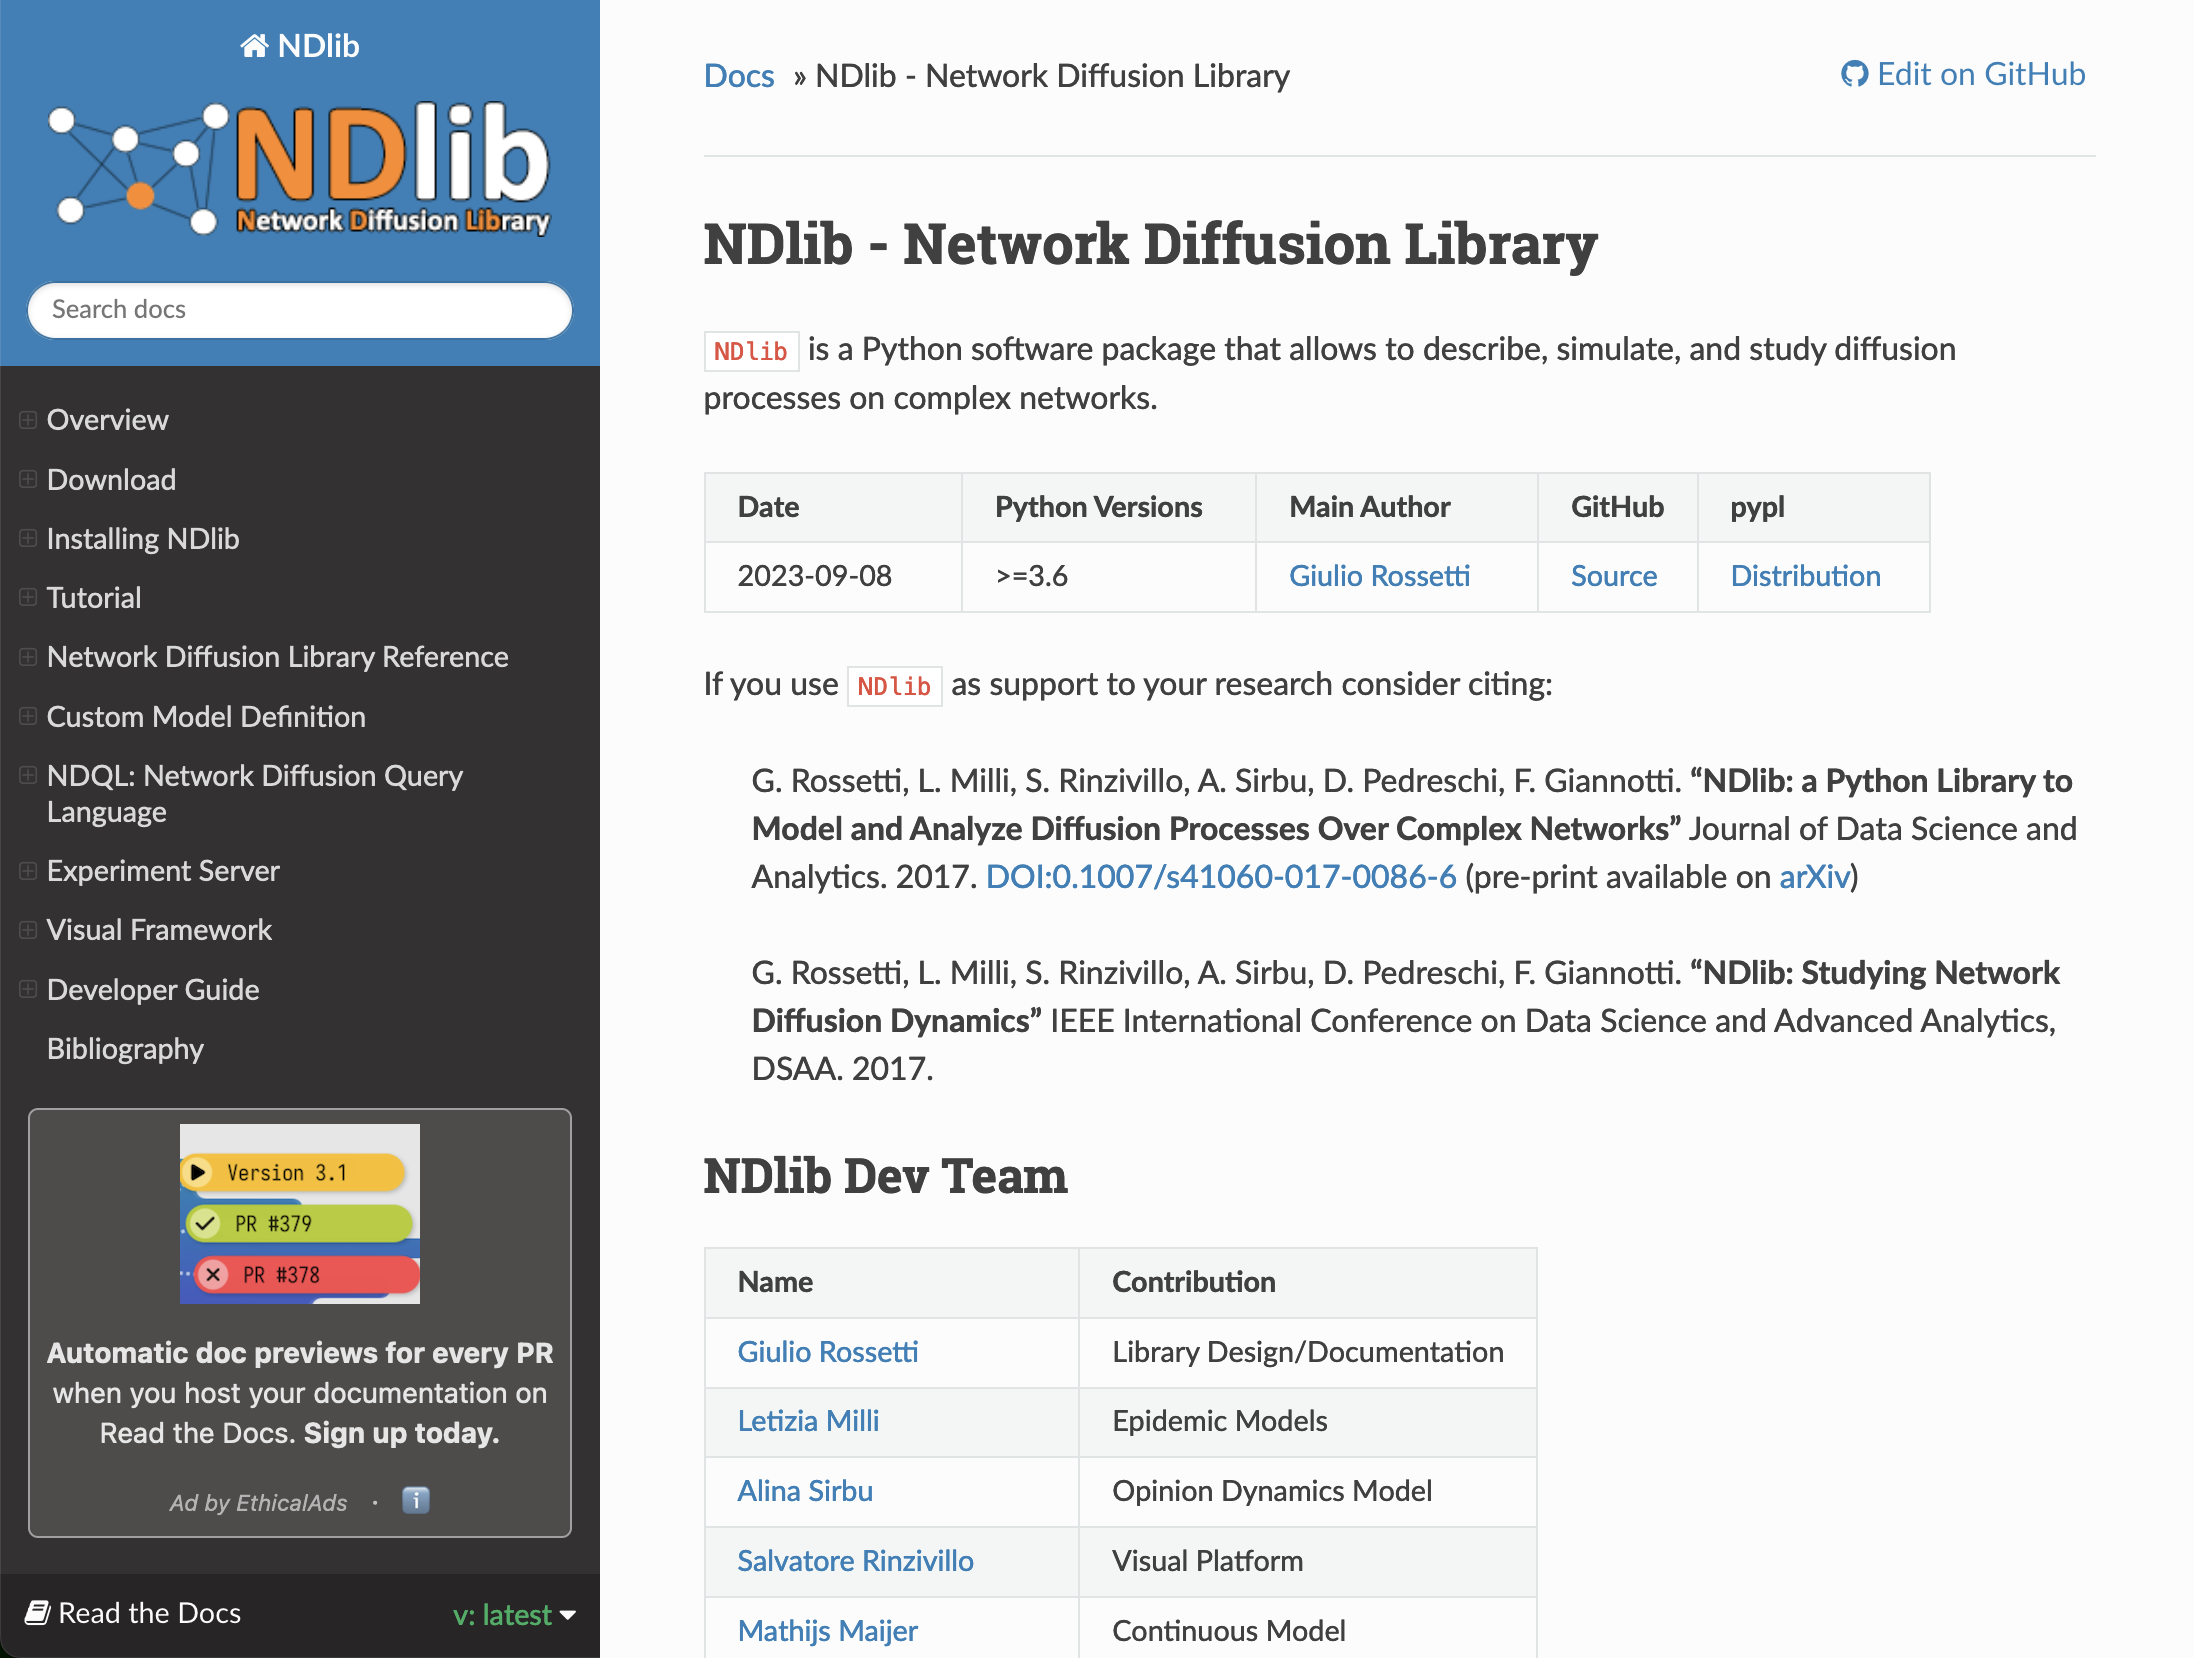
\includegraphics[width=1\textwidth]{figures/ndlib.png}
                \caption{NDlib's website.}
            \end{figure}
        \end{column}
    \end{columns}
\end{frame}

\begin{frame}{\secname}
    However, if we consider more complex...\\
    \vspace{1em}
    \hspace{3em}...network models \textcolor{gray}{(e.g. multilayer graphs)}... \\
    \vspace{1em}
    \hspace{3em}...diffusion models \textcolor{gray}{(e.g. spreading of coexisting processes)}... \\
    \vspace{1em}
    \hspace{10em}...\textbf{a gap among the available toolkits} emerges.
\end{frame}

\begin{frame}{\secname}
    \begin{center}
        For instance, which library should we choose if we have to * ?
    \end{center}
    \vspace{3em}
    \begin{itemize}
        \setlength{\itemindent}{-2em}
        \item[] * model simultaneous spreading of opinions about advertised products
        \item[] * convert dataset of interactions into a temporal graph
        \item[] * process a multilayer network to extract its centrality measures
        \item[] * identify super spreaders in a multiplex network under ICM
    \end{itemize}
\end{frame}

% \begin{frame}{\secname}
%     \onslide<1->{My research group works on problems related to multilayer/temporal networks,
%     spreading phenomena, influence maximisation, data streams, etc.}
%     \onslide<2->{\begin{center}
%         \arrowdown
%     \end{center}
%     As a result of our recent activities, we decided to merge and wrap up a code we developed into
%     a reusable library and to share it with the community as an attempt of filling the gap in.}
%     \onslide<3->{\begin{center}
%         \arrowdown
%     \end{center}
%     The main permises under which we operated are:
%     \begin{enumerate}
%         \item<3-> support both for multilayer and temporal networks,
%         \item<4-> support for spreading models with discrete states,
%         \item<5-> compatibility with other tools commonly used in network science,
%         \item<6-> releasing a tool in form of a framework with open interfaces.
%     \end{enumerate}}
% \end{frame}

\begin{frame}{\secname}
    \onslide<1->{My research group works on problems related to multilayer/temporal networks,
    spreading phenomena, influence maximisation, data streams, etc.}
    \onslide<2->{\begin{center}
        \arrowdown
    \end{center}
    During the research, we produced a code that can be reused as a boilerplate for further
    experiments, with interfaces allowing anyone to quickly implement a custom spreading model.}
    \onslide<3->{\begin{center}
        \arrowdown
    \end{center}
    With regard to the observed gap among existing toolkits, we decided to merge and wrap the code
    into a library to share it with the community as a small contribution to make experiments easier.}
\end{frame}

\section{Key Features of \lstinline[style=py]{network-diffusion}}

\begin{frame}{\secname}
    Functionalities of the library:
    \vspace{1em}
    \begin{itemize}[<+->]
        \item end-to-end workflow for simulations of spreading phenomena,
        \item predefined (basic) spreading models,
        \item an interface for implementing custom discrete spreading models,
        \item support for temporal networks (CogSNet and snapshot-based),
        \item support for the multilayer networks,
        \item most of centrality metrics extended to multilayer networks.
    \end{itemize}
\end{frame}

\begin{frame}{\secname}
    Environmental requirements/features:
    \vspace{1em}
    \begin{itemize}
        \item released under MIT licence,
        \item support for Linux, macOS, and Windows\footnote{Although we develop and use it mostly on Unix OSs},
        \item Python >= 3.10 compatibility,
        \item C snippets in the CogSNet module to speed-up computations,
        \item NetworkX compatibility.
    \end{itemize}
\end{frame}

% \begin{frame}[fragile]{\secname}
%     To prepare the experiment we have to provide: \textbf{a network}, \textbf{a spreading model} and \textbf{auxiliary parameters}.
%     Then, the simulation unfolds as follows:
%     \vspace{1em}
%     \begin{algorithmic}[1]
%         \Procedure{\lstinline[style=py]{perform_propagation}}{\lstinline[style=py]{network, model, epochs*}}
%         \State \lstinline[style=py]{states_0} $\gets$ \lstinline[style=py]{model.determine_initial_states()}
%         \State \lstinline[style=py]{model.update_network(states_0)} % \Comment{Predefined function in the \texttt{BaseModel} class}
%         \For{\lstinline[style=py]{e} in \lstinline[style=py]{[1, ..., epochs]}}
%         \State \quad \quad \lstinline[style=py]{states_e} $\gets$ \lstinline[style=py]{model.network_evaluation_step(network)}
%         \State \quad \quad \lstinline[style=py]{model.update_network(network, states_e)}
%         \EndFor
%         \State \lstinline[style=py]{logs} $\gets$ generate logs from experiment \\
%         \Return \lstinline[style=py]{logs}
%         \EndProcedure
%     \end{algorithmic}
% \end{frame}

\section{Example I - Predefined Model}

\begin{frame}{\secname}
    In this example, we will see how to trigger spread under the Linear Threshold Model in a toy,
    multilayer network.
    \begin{block}{Linear Threshold Model}
    Each node:
    \begin{itemize}
        \item can fall in two states: \textit{active} and \textit{inactive},
        \item becomes \textit{active} if the fraction of its \textit{active} neighbors to all neighbours
        exceeds certain threshold.
    \end{itemize}
    \end{block}
    In case of multilayer networks the actors not the nodes\footnote{which can be considered as avatars
    of the actors on the network's layers} are a subject of the diffusion. Thus, we have to define
    how to aggregate impulses from the layers. In this example we will consider "OR" strategy.
    % which says that the actor can be activated if any of nodes representing it in the network gets activated.
\end{frame}

\begin{frame}{\secname}
    \begin{figure}
        \centering
        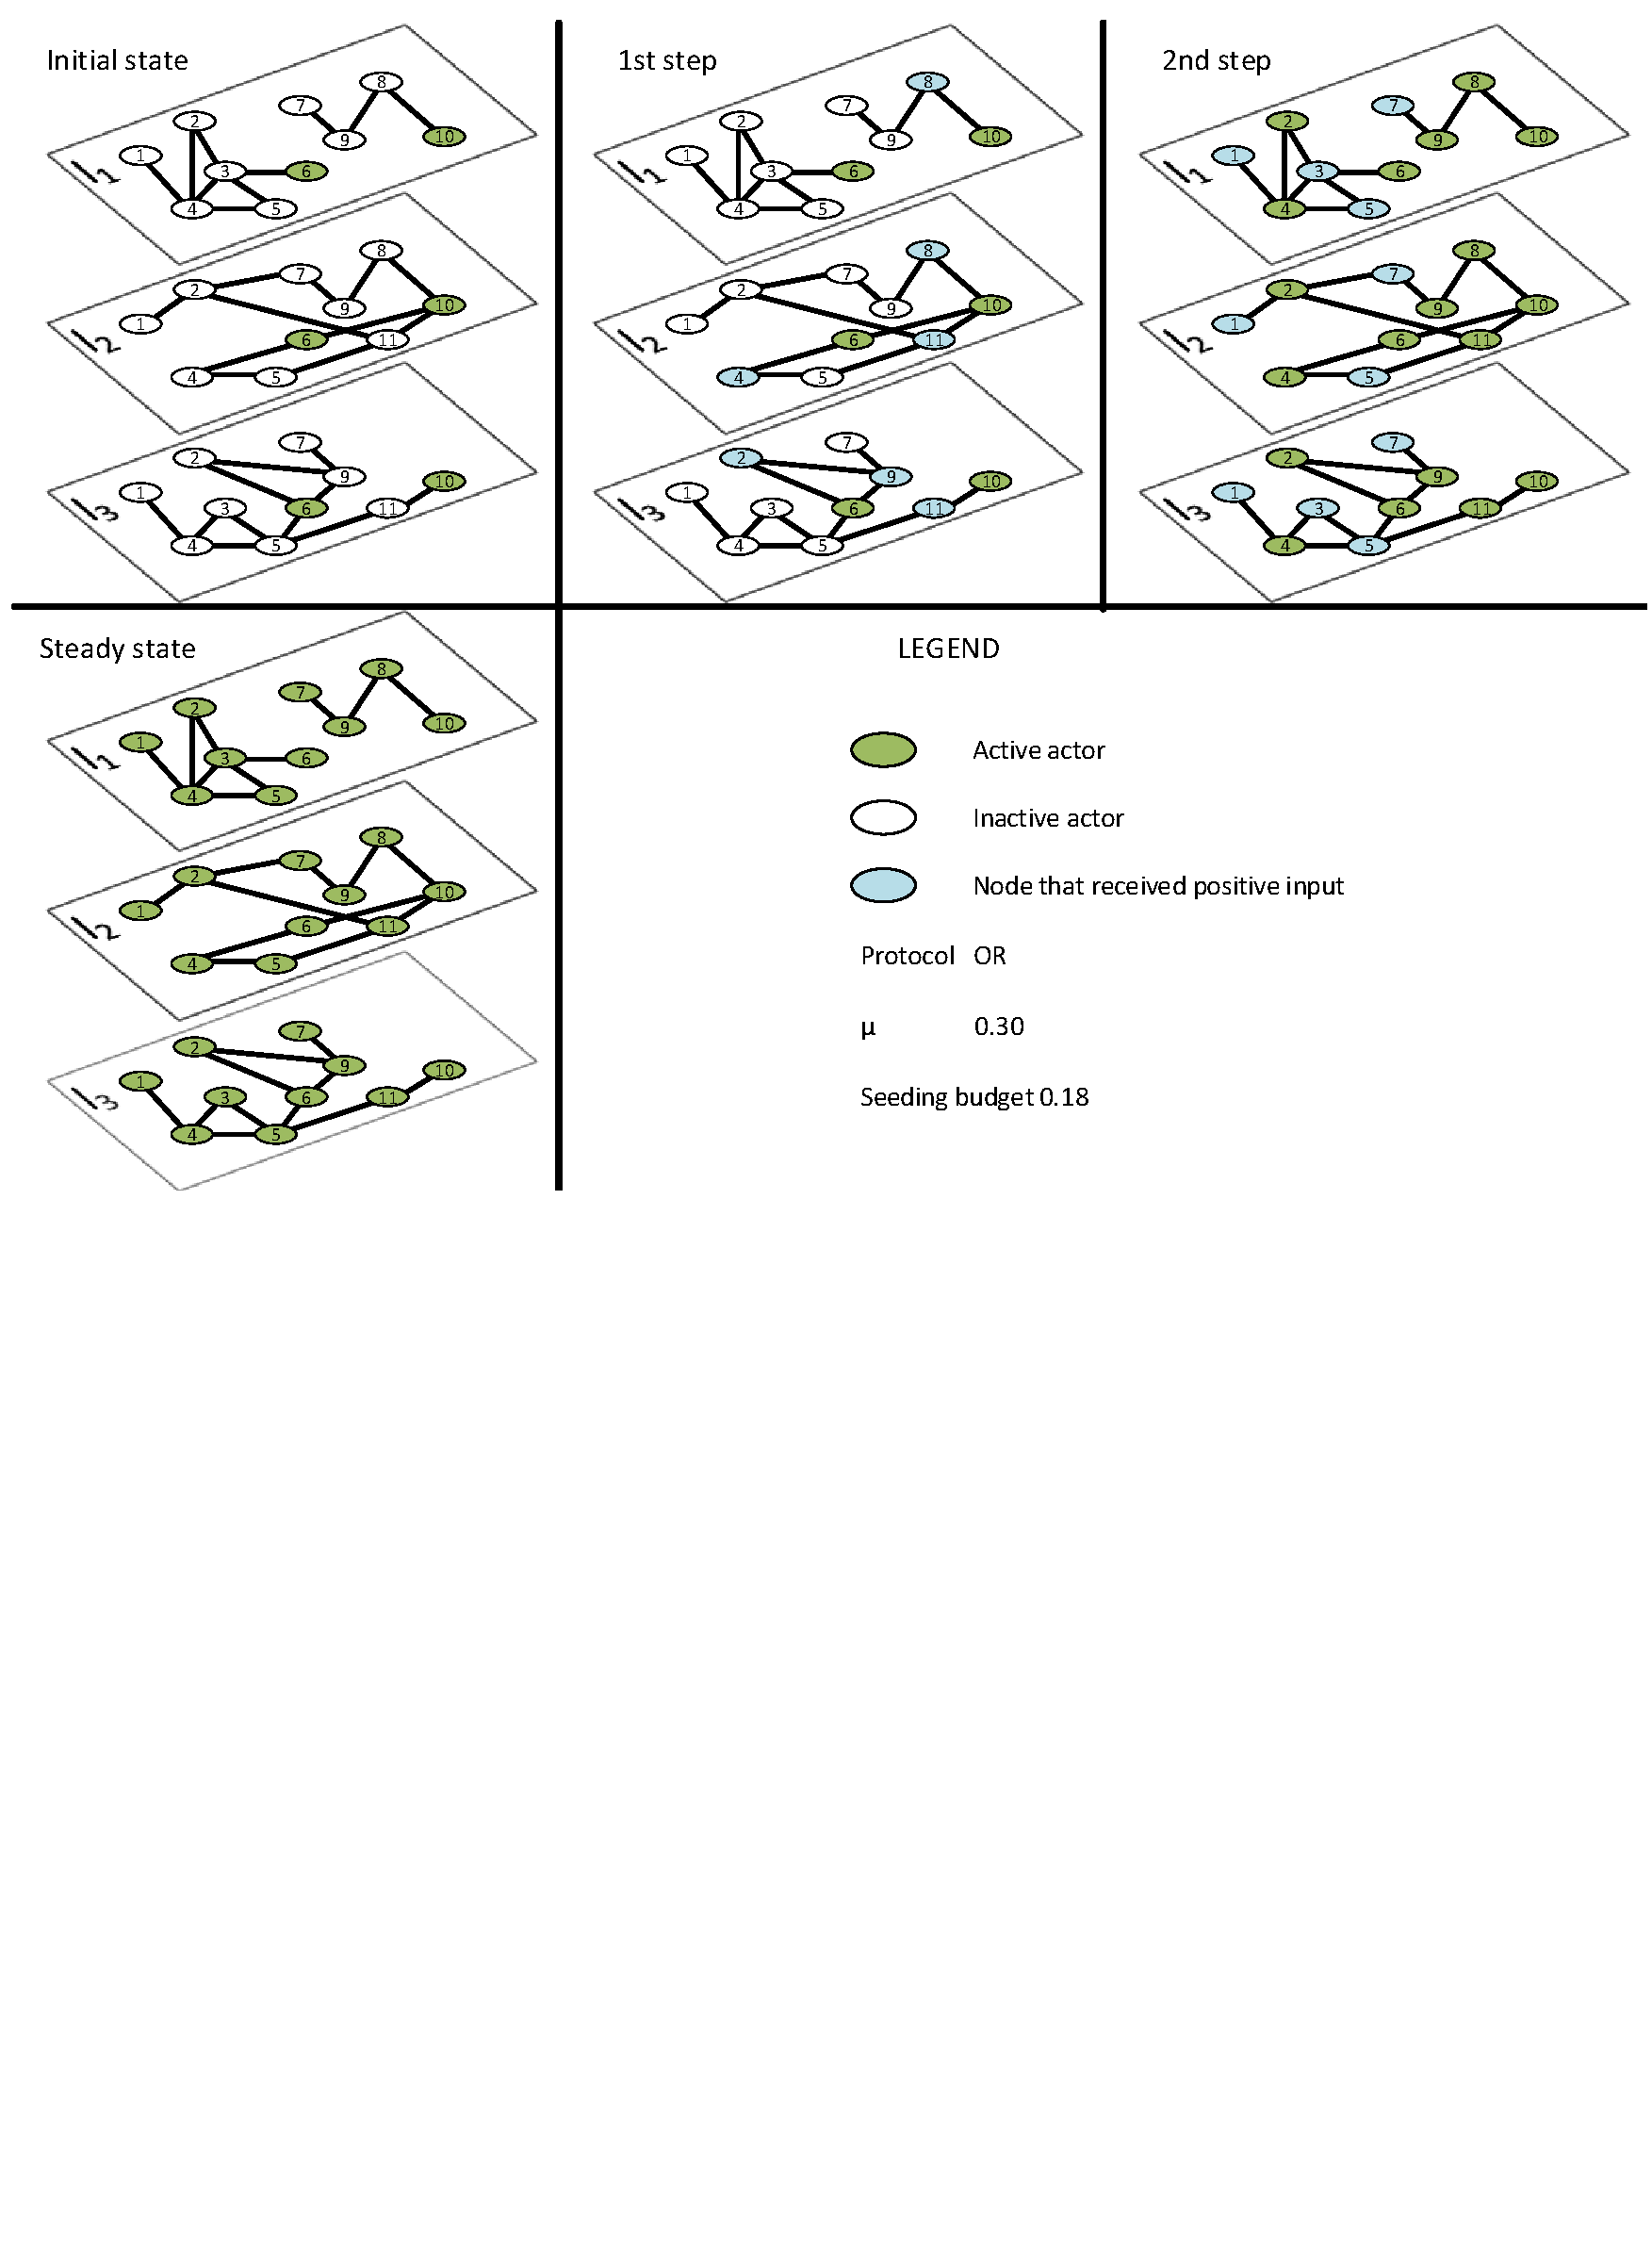
\includegraphics[width=.75\textwidth]{figures/ltm_example_or.pdf}
        \caption{Propagation according to LTM with the $OR$ strategy in a multilayer network -
        active actors: seeds $\{6, 10\}$, in a stable state: all of them.}
    \end{figure}
\end{frame}

\begin{frame}{\secname}
    \begin{center}
        \large Let's model this problem with \lstinline[style=py]{network-diffusion}!
    \end{center}
\end{frame}

\section{Example II - Custom Model}

\begin{frame}{\secname}
    In this example we will consider a joint disease-awareness model (SIR-UA) that can be used e.g.
    to assess the effectiveness of various countermeasures against the spread of COVID-19:
    \begin{columns}[T]
        \captionsetup{font=scriptsize}
        \begin{column}{.5\textwidth}
            \begin{table}
            \centering
            \caption{Transition weights with explanation.}
            \resizebox{.7\textwidth}{!}{%
            \begin{tabular}{c|p{4cm}}
            Symbol & Description \\ \hline
            $\alpha$ & probability of infection for unaware agents \\ \hline
            $\alpha'$ & probability of infection for aware agents \\ \hline
            $\beta$ & probability of recovery \\ \hline
            $\gamma$ & probability of awareness for uninfected agents \\ \hline
            $\delta$& probability of awareness for infected agents \\
            \end{tabular}%
            }
            \end{table}
        \end{column}
        \begin{column}{0.5\textwidth}
        \begin{figure}
            \centering
            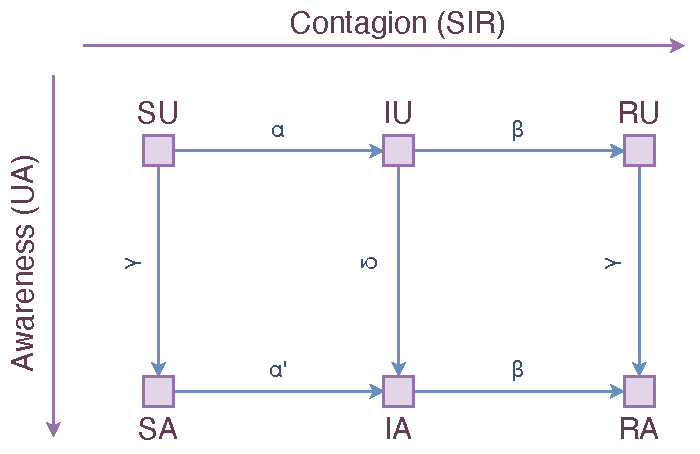
\includegraphics[width=\textwidth]{figures/sir_ua.pdf}
            \caption{State and transition graph for SIR-UA.}
        \end{figure}
        \end{column}
      \end{columns}
\end{frame}

\begin{frame}{\secname}
    To create an own spreading model, we have to extend the abstract base class
    (\lstinline[style=py]{nd.models.BaseModel}) by implementing:
    \begin{itemize}
        \item a field \lstinline[style=py]{_compartmental_graph},
        \item a field \lstinline[style=py]{_seed_selector},
        \item a method \lstinline[style=py]{determine_initial_states},
        \item a method \lstinline[style=py]{agent_evaluation_step},
        \item a method \lstinline[style=py]{network_evaluation_step},
        \item methods \lstinline[style=py]{__str__} and \lstinline[style=py]{get_allowed_states}.
    \end{itemize}
    \vspace{1em}
    The following entities (with implemented method \lstinline[style=py]{update_network}) are
    utilised in the class \lstinline[style=py]{nd.Simulator} which orchestrates the experiment.
\end{frame}

\begin{frame}{\secname}
    \begin{center}
        \large Let's model this problem with \lstinline[style=py]{network-diffusion}!
    \end{center}
\end{frame}

\section{Resources and References}

\begin{frame}[fragile]{\secname}
    The library can be installed with:
    \begin{center}
        \large
        \begin{verbatim}
            pip install network-diffusion
        \end{verbatim}
    \end{center}
    We have also published other useful resources:
    \begin{itemize}[<+->]
        \item PyPI website: \url{pypi.org/project/network-diffusion},
        \item GitHub page: \url{github.com/anty-filidor/network_diffusion},
        \item Reference guide: \url{network-diffusion.readthedocs.io},
        \item Paper with more use-cases presented: \url{arxiv.org/abs/2405.18085}.
    \end{itemize}
\end{frame}

\section{Limitations of \lstinline[style=py]{network-diffusion}}

\begin{frame}{\secname}
    There is still some work to do...
    \vspace{1em}
    \begin{itemize}
        \item computational performance can be better,
        \item we are limited to discrete spreading models,
        \item we cannot model agent's complex states (e.g. internal/external),
        \item much less pre-defined spreading models than in NDlib,
        \item library maintenance guaranteed up to my graduation \Winkey.
    \end{itemize}
\end{frame}

\begin{frame}[allowframebreaks]
    \frametitle{References}
    \printbibliography
\end{frame}

\addtocounter{framenumber}{1}

\end{document}
